\documentclass[a4paper,showframe,11pt]{report}\usepackage[]{graphicx}\usepackage[]{color}
%% maxwidth is the original width if it is less than linewidth
%% otherwise use linewidth (to make sure the graphics do not exceed the margin)
\makeatletter
\def\maxwidth{ %
  \ifdim\Gin@nat@width>\linewidth
    \linewidth
  \else
    \Gin@nat@width
  \fi
}
\makeatother

\definecolor{fgcolor}{rgb}{0.196, 0.196, 0.196}
\newcommand{\hlnum}[1]{\textcolor[rgb]{0.063,0.58,0.627}{#1}}%
\newcommand{\hlstr}[1]{\textcolor[rgb]{0.063,0.58,0.627}{#1}}%
\newcommand{\hlcom}[1]{\textcolor[rgb]{0.588,0.588,0.588}{#1}}%
\newcommand{\hlopt}[1]{\textcolor[rgb]{0.196,0.196,0.196}{#1}}%
\newcommand{\hlstd}[1]{\textcolor[rgb]{0.196,0.196,0.196}{#1}}%
\newcommand{\hlkwa}[1]{\textcolor[rgb]{0.231,0.416,0.784}{#1}}%
\newcommand{\hlkwb}[1]{\textcolor[rgb]{0.627,0,0.314}{#1}}%
\newcommand{\hlkwc}[1]{\textcolor[rgb]{0,0.631,0.314}{#1}}%
\newcommand{\hlkwd}[1]{\textcolor[rgb]{0.78,0.227,0.412}{#1}}%
\let\hlipl\hlkwb

\usepackage{framed}
\makeatletter
\newenvironment{kframe}{%
 \def\at@end@of@kframe{}%
 \ifinner\ifhmode%
  \def\at@end@of@kframe{\end{minipage}}%
  \begin{minipage}{\columnwidth}%
 \fi\fi%
 \def\FrameCommand##1{\hskip\@totalleftmargin \hskip-\fboxsep
 \colorbox{shadecolor}{##1}\hskip-\fboxsep
     % There is no \\@totalrightmargin, so:
     \hskip-\linewidth \hskip-\@totalleftmargin \hskip\columnwidth}%
 \MakeFramed {\advance\hsize-\width
   \@totalleftmargin\z@ \linewidth\hsize
   \@setminipage}}%
 {\par\unskip\endMakeFramed%
 \at@end@of@kframe}
\makeatother

\definecolor{shadecolor}{rgb}{.97, .97, .97}
\definecolor{messagecolor}{rgb}{0, 0, 0}
\definecolor{warningcolor}{rgb}{1, 0, 1}
\definecolor{errorcolor}{rgb}{1, 0, 0}
\newenvironment{knitrout}{}{} % an empty environment to be redefined in TeX

\usepackage{alltt}
\usepackage{standalone}
\standalonetrue
\ifstandalone
  \usepackage{../../haziq_thesis}
  \usepackage{../../haziq_maths}
  \usepackage{../../haziq_glossary}
  \addbibresource{../../bib/haziq.bib}
  \externaldocument{../01/.texpadtmp/introduction}
  \externaldocument{../02/.texpadtmp/chapter2}
  \externaldocument{../03/.texpadtmp/chapter3}
  \externaldocument{../04/.texpadtmp/chapter4}  % remove this
  \externaldocument{../appendix/.texpadtmp/appendix}
\fi




\IfFileExists{upquote.sty}{\usepackage{upquote}}{}
\begin{document}

% \section{Examples}  % remove this

We demonstrate I-prior modelling on a toy data set to illustrate the Nyström method, as well as three other real-data examples.
All of the analyses were conducted in \proglang{R}, and I-prior model estimation was done using the \pkg{iprior} package.
In all of these examples, \ref{ass:A1}--\ref{ass:A3} were assumed.

\subsection[Using the Nystrom method]{Using the Nystr\"om method}

We investigate the use of the Nystr\"om method of approximating the kernel matrix in estimating I-prior models.
Let us revisit the data set generated by \cref{eq:examplesmoothingdata} described in \cref{sec:compareestimation}.
The features of this regression function are two large bumps at the centres of the mixed Gaussian PDFs, and also a small bump right after $x>4.5$ caused by the additional exponential function.
The true regression function tends to positive infinity as $x$ increases, and to zero as $x$ decreases.
Samples of $(x_i,y_i)$, $i=1,\dots,2000$ have been generated by the built-in \code{gen_smooth()} function, of which the first few lines of the data are shown below.

\begin{knitrout}
\definecolor{shadecolor}{rgb}{1, 1, 1}\color{fgcolor}\begin{kframe}
\begin{alltt}
\hlstd{R> }\hlstd{dat} \hlkwb{<-} \hlkwd{gen_smooth}\hlstd{(}\hlkwc{n} \hlstd{=} \hlnum{2000}\hlstd{,} \hlkwc{xlim} \hlstd{=} \hlkwd{c}\hlstd{(}\hlopt{-}\hlnum{1}\hlstd{,} \hlnum{5.5}\hlstd{),} \hlkwc{seed} \hlstd{=} \hlnum{1}\hlstd{)}
\hlstd{R> }\hlkwd{head}\hlstd{(dat)}
\end{alltt}
\begin{verbatim}
##            y         X
## 1  0.6803514 -2.608953
## 2  3.6747031 -2.554039
## 3 -1.1563508 -2.381275
## 4  2.2657657 -2.280259
## 5  2.5398243 -2.214122
## 6  1.2929592 -2.170532
\end{verbatim}
\end{kframe}
\end{knitrout}

One could fit the regression model using all available data points, with an I-prior from the fBm-0.5 RKHS of functions as follows (note that the \code{silent} option is used to suppress the output from the \code{iprior()} function):

\begin{knitrout}
\definecolor{shadecolor}{rgb}{1, 1, 1}\color{fgcolor}\begin{kframe}
\begin{alltt}
\hlstd{R> }\hlstd{(mod.full} \hlkwb{<-} \hlkwd{iprior}\hlstd{(y} \hlopt{~} \hlstd{X, dat,} \hlkwc{kernel} \hlstd{=} \hlstr{"fbm"}\hlstd{,}
\hlstd{+  }                    \hlkwc{control} \hlstd{=} \hlkwd{list}\hlstd{(}\hlkwc{silent} \hlstd{=} \hlnum{TRUE}\hlstd{)))}
\end{alltt}
\begin{verbatim}
## Log-likelihood value: -4355.075 
## 
##  lambda     psi 
## 2.30244 0.23306
\end{verbatim}
\end{kframe}
\end{knitrout}

To implement the Nystr\"om method, the option \code{nystrom = 50} was added to the above function call, which uses 50 randomly selected data points for the Nystr\"om approximation.

\begin{knitrout}
\definecolor{shadecolor}{rgb}{1, 1, 1}\color{fgcolor}\begin{kframe}
\begin{alltt}
\hlstd{R> }\hlstd{(mod.nys} \hlkwb{<-} \hlkwd{iprior}\hlstd{(y} \hlopt{~} \hlstd{X, dat,} \hlkwc{kernel} \hlstd{=} \hlstr{"fbm"}\hlstd{,} \hlkwc{nystrom} \hlstd{=} \hlnum{50}\hlstd{,}
\hlstd{+  }                   \hlkwc{control} \hlstd{=} \hlkwd{list}\hlstd{(}\hlkwc{silent} \hlstd{=} \hlnum{TRUE}\hlstd{)))}
\end{alltt}
\begin{verbatim}
## Log-likelihood value: -1945.33 
## 
##  lambda     psi 
## 1.64833 0.13538
\end{verbatim}
\end{kframe}
\end{knitrout}

The hyperparameters estimated for both models are slightly different.
The log-likelihood is also different, but this is attributed to information loss due to the approximation procedure.
Nevertheless, we see from \cref{fig:nystrom.plot} that the estimated regression functions are quite similar in both the full model and the approximated model.
The main difference is that the the Nystr\"om method was not able to extrapolate the right hand side of the plot well, because it turns out that there were no data points used from this region.
This can certainly be improved by using a more intelligent sampling scheme.
The full model took a little over 12 minutes to converge, while the Nystr\"om method took seconds without compromising too much on root mean squared error of predictions.
Storage savings is significantly higher with the Nystr\"om method as well.

\begin{knitrout}
\definecolor{shadecolor}{rgb}{1, 1, 1}\color{fgcolor}\begin{kframe}
\begin{alltt}
\hlstd{R> }\hlkwd{get_time}\hlstd{(mod.full);} \hlkwd{get_size}\hlstd{(mod.full,} \hlstr{"MB"}\hlstd{);} \hlkwd{get_prederror}\hlstd{(mod.full)}
\end{alltt}
\begin{verbatim}
## 12.10819 mins
## 128.2 MB
## Training RMSE 
##      2.054232
\end{verbatim}
\begin{alltt}
\hlstd{R> }\hlkwd{get_time}\hlstd{(mod.nys);} \hlkwd{get_size}\hlstd{(mod.nys);} \hlkwd{get_prederror}\hlstd{(mod.nys)}
\end{alltt}
\begin{verbatim}
## 1.287808 secs
## 982.2 kB
## Training RMSE 
##      2.171928
\end{verbatim}
\end{kframe}
\end{knitrout}

\begin{knitrout}
\definecolor{shadecolor}{rgb}{1, 1, 1}\color{fgcolor}\begin{figure}[htb]

{\centering 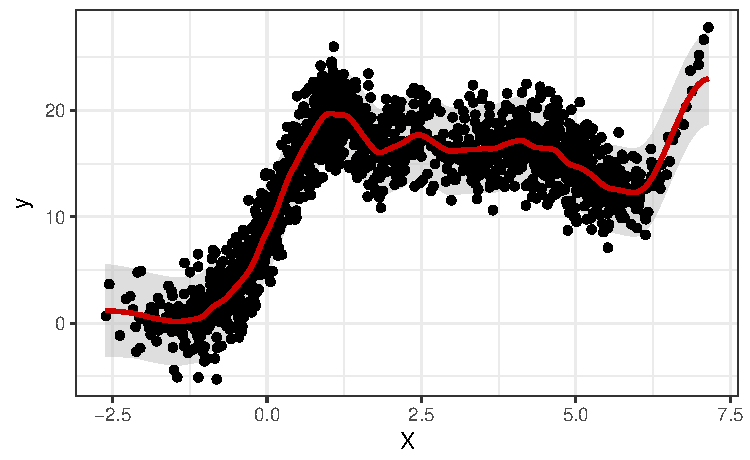
\includegraphics[width=0.85\textwidth]{figure/04-nystrom_plot-1} 
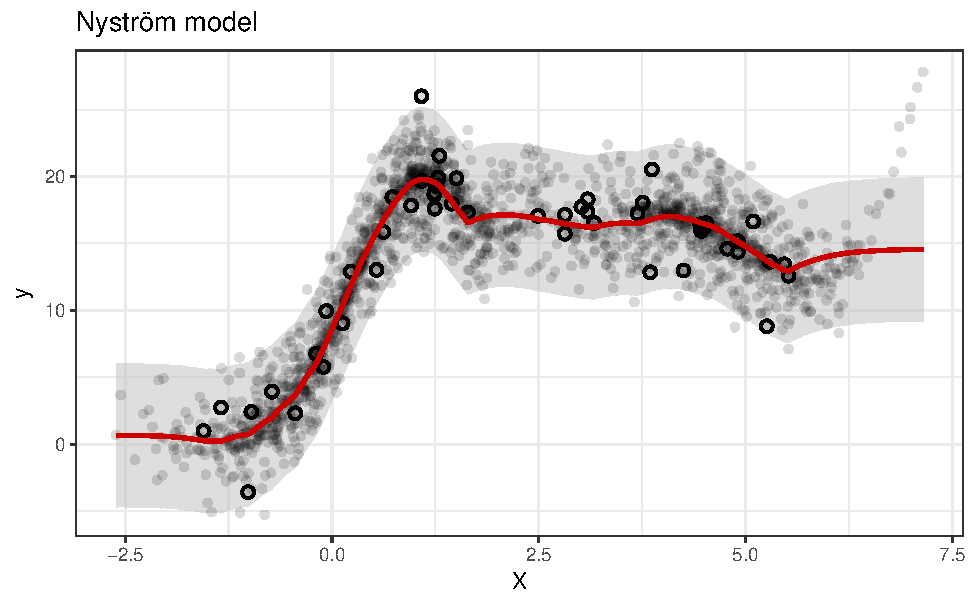
\includegraphics[width=0.85\textwidth]{figure/04-nystrom_plot-2} 

}

\caption[Plot of predicted regression function for the full model (top) and the Nystr\"om approximated method (bottom)]{Plot of predicted regression function for the full model (top) and the Nystr\"om approximated method (bottom). For the Nystr\"om plot, the data points that were active are shown by circles with bold outlines.}\label{fig:nystrom.plot}
\end{figure}


\end{knitrout}
% out.width = "0.49\\textwidth", fig.width = 5, fig.height = 5 * 4 / 6.5,

\subsection{Random effects models}

In this section, a comparison between a standard random effects model and the I-prior approach for estimating varying intercept and slopes model is illustrated.
The example concerns control data\footnotemark\ from several runs of radioimmunoassays (RIA) for the protein insulin-like growth factor (IGF-I) (explained in further detail in \cite[§3.2.1]{davidian1995nonlinear}).
RIA is an in vitro assay technique which is used to measure concentration of antigens---in our case, the IGF-I proteins.
When an RIA is run, control samples at known concentrations obtained from a particular lot are included for the purpose of assay quality control.
It is expected that the concentration of the control material remains stable as the machine is used, up to a maximum of about 50 days, at which point  control samples from a new batch is used to avoid degradation in assay performance.

\begin{knitrout}
\definecolor{shadecolor}{rgb}{1, 1, 1}\color{fgcolor}\begin{kframe}
\begin{alltt}
\hlstd{R> }\hlkwd{data}\hlstd{(IGF,} \hlkwc{package} \hlstd{=} \hlstr{"nlme"}\hlstd{)}
\hlstd{R> }\hlkwd{head}\hlstd{(IGF)}
\end{alltt}
\begin{verbatim}
## Grouped Data: conc ~ age | Lot
##   Lot age conc
## 1   1   7 4.90
## 2   1   7 5.68
## 3   1   8 5.32
## 4   1   8 5.50
## 5   1  13 4.94
## 6   1  13 5.19
\end{verbatim}
\end{kframe}
\end{knitrout}

\footnotetext{This data is available in the \proglang{R} package \pkg{nlme} \citep{nlme}.}

The data consists of IGF-I concentrations (\code{conc}) from control samples from 10 different lots measured at differing \code{age}s of the lot.
The data were collected with the aim of identifying possible trends in control values \code{conc} with \code{age}, ultimately investigating whether or not the usage protocol of maximum sample age of 50 days is justified.
\citet{pinheiro2000mixed} remarks that this is not considered a longitudinal problem because different samples were used at each measurement.

We shall  model the IGF data set using the I-prior methodology using the ANOVA-decomposed regression function
%
\[
  f(\texttt{age}, \texttt{Lot}) = f_1(\texttt{age}) + f_2(\texttt{Lot}) + f_{12}(\texttt{age}, \texttt{Lot})
\]
%
where $f_1$ lies in the linear RKHS $\cF_1$, $f_2$ in the Pearson RKHS $\cF_2$ and $f_{12}$ in the tensor product space $\cF_{12} = \cF_1 \otimes \cF_2$.
The regression function $f$ then lies in the RKHS $\cF = \cF_1 \oplus \cF_2 \oplus \cF_{12}$ with kernel equal to the sum of the kernels from each of the RKHSs.
The explanation here is that the \code{conc} levels are assumed to be related to both \code{age} and \code{Lot}, and in particular, the contribution of \code{age} on \code{conc} varies with each individual \code{Lot}.
This gives the intended effect of a linear mixed-effects model, which is thought to be suitable in this case, in order to account for within-lot and between-lot variability.
We first fit the model using the \pkg{iprior} package, and then compare the results with the standard random effects model using the \proglang{R} command \code{lme4::lmer()}.
The command to fit the I-prior model using the EM algorithm is

\begin{knitrout}
\definecolor{shadecolor}{rgb}{1, 1, 1}\color{fgcolor}\begin{kframe}
\begin{alltt}
\hlstd{R> }\hlstd{mod.iprior} \hlkwb{<-} \hlkwd{iprior}\hlstd{(conc} \hlopt{~} \hlstd{age} \hlopt{*} \hlstd{Lot, IGF,} \hlkwc{method} \hlstd{=} \hlstr{"em"}\hlstd{)}
\end{alltt}
\begin{verbatim}
## ========================================
## Converged after 57 iterations.
\end{verbatim}
\begin{alltt}
\hlstd{R> }\hlkwd{summary}\hlstd{(mod.iprior)}
\end{alltt}
\begin{verbatim}
## Call:
## iprior(formula = conc ~ age * Lot, data = IGF, method = "em")
## 
## RKHS used:
## Linear (age)
## Pearson (Lot)
## 
## Residuals:
##    Min. 1st Qu.  Median 3rd Qu.    Max. 
## -4.4889 -0.3798 -0.0090  0.2563  4.3973 
## 
## Hyperparameters:
##           Estimate   S.E.      z P[|Z>z|]    
## lambda[1]   0.0000 0.0002 -0.004    0.997    
## lambda[2]   0.0007 0.0030  0.238    0.812    
## psi         1.4576 0.1366 10.672   <2e-16 ***
## ---
## Signif. codes:  0 '***' 0.001 '**' 0.01 '*' 0.05 '.' 0.1 ' ' 1
## 
## Closed-form EM algorithm. Iterations: 57/100 
## Converged to within 1e-08 tolerance. Time taken: 2.882966 secs
## Log-likelihood value: -291.9033 
## RMSE of prediction: 0.8273639 (Training)
\end{verbatim}
\end{kframe}
\end{knitrout}
\begin{knitrout}
\definecolor{shadecolor}{rgb}{1, 1, 1}\color{fgcolor}\begin{figure}

{\centering 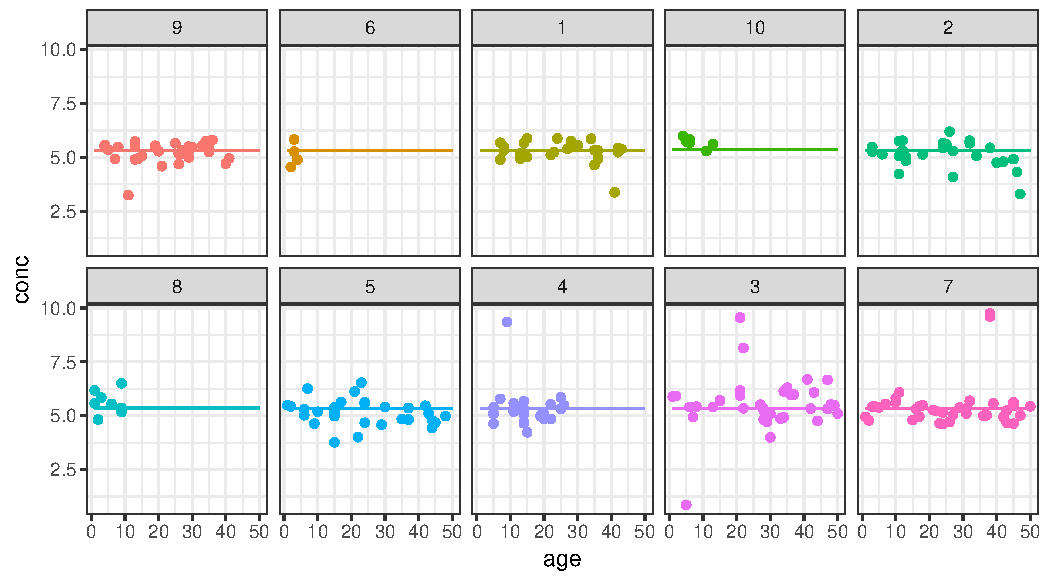
\includegraphics[width=\maxwidth]{figure/04-IGF_mod_iprior_plot-1} 

}

\caption[Plot of fitted regression line for the I-prior model on the IGF data set, separated into each of the 10 lots]{Plot of fitted regression line for the I-prior model on the IGF data set, separated into each of the 10 lots.}\label{fig:IGF.mod.iprior.plot}
\end{figure}


\end{knitrout}

To make inference on the covariates, we look at the scale parameters \code{lambda}.
We see that both scale parameters for \code{age} and \code{Lot} are close to zero, and a test of significance is not able to reject the hypothesis that these parameters are indeed null.
We conclude that neither \code{age} nor \code{Lot} has a linear effect on the \code{conc} levels.
The plot of the fitted regression line in \cref{fig:IGF.mod.iprior.plot} does show an almost horizontal line for each \code{Lot}.
% Another way of looking at this problem is to compare the fitted model with a constant model, i.e., a model with only the intercept fitted.
% This model is able to be fitted by constraining and the \code{lambda} parameters to zero, as follows:

% <IGF.mod.iprior.const, cache = TRUE>>=
% @

% We then perform a log-likelihood ratio test to compare the two models.
% The test statistic yields a value of round(D) which follows an asymptotic $\chi^2$ distribution with two degrees of freedom (three parameters estimated in the original model, and only one in the constant model).

%\newpage
The standard random effects model, as explored by \citet{davidian1995nonlinear} and \citet{pinheiro2000mixed}, is
%
\begin{align*}
  \begin{gathered}
    \texttt{conc}_{ij} = \beta_{0j} + \beta_{1j}\texttt{age}_{ij} + \epsilon_{ij} \\
    \begin{pmatrix}
      \beta_{0j} \\
      \beta_{1j} \\
    \end{pmatrix}
    \sim \N \left(
      \begin{pmatrix}
        \beta_{0} \\
        \beta_{1} \\
      \end{pmatrix},
      \begin{pmatrix}
        \sigma_{0}^2 & \sigma_{01} \\
        \sigma_{01}  & \sigma_1^2 \\
      \end{pmatrix}
    \right) \\
    \epsilon_{ij} \sim \N(0, \sigma^2) \\
  \end{gathered}
\end{align*}
%
for $i=1,\dots,n_j$ and the index $j$ representing the 10 \code{Lots}.
Fitting this model using \code{lmer}, we can test for the significance of the fixed effect $\beta_0$, for which we find that it is not ($p$-value = 0.616), and arrive at the same conclusion as in the I-prior model.
However, we notice that the package reports a perfect negative correlation between the random effects, $\sigma_{01}$.
This indicates a potential numerical issue when fitting the model---a value of exactly $-1$, $0$ or $1$ is typically imposed by the package to force through estimation in the event of non-positive definite covariance matrices arising.
We can inspect the eigenvalues of the covariance matrix for the random effects to check that they are indeed non-positive definite.

\begin{knitrout}
\definecolor{shadecolor}{rgb}{1, 1, 1}\color{fgcolor}\begin{kframe}
\begin{alltt}
\hlstd{R> }\hlstd{(mod.lmer} \hlkwb{<-} \hlkwd{lmer}\hlstd{(conc} \hlopt{~} \hlstd{age} \hlopt{+} \hlstd{(age} \hlopt{|} \hlstd{Lot), IGF))}
\end{alltt}
\begin{verbatim}
## Linear mixed model fit by REML ['lmerMod']
## Formula: conc ~ age + (age | Lot)
##    Data: IGF
## REML criterion at convergence: 594.3662
## Random effects:
##  Groups   Name        Std.Dev. Corr 
##  Lot      (Intercept) 0.082507      
##           age         0.008092 -1.00
##  Residual             0.820628      
## Number of obs: 237, groups:  Lot, 10
## Fixed Effects:
## (Intercept)          age  
##    5.374974    -0.002535
\end{verbatim}
\begin{alltt}
\hlstd{R> }\hlkwd{eigen}\hlstd{(}\hlkwd{VarCorr}\hlstd{(mod.lmer)}\hlopt{$}\hlstd{Lot)}
\end{alltt}
\begin{verbatim}
## eigen() decomposition
## $values
## [1]  6.872939e-03 -1.355253e-20
## 
## $vectors
##             [,1]        [,2]
## [1,] -0.99522490 -0.09760839
## [2,]  0.09760839 -0.99522490
\end{verbatim}
\end{kframe}
\end{knitrout}

\begin{knitrout}
\definecolor{shadecolor}{rgb}{1, 1, 1}\color{fgcolor}\begin{figure}[t]

{\centering 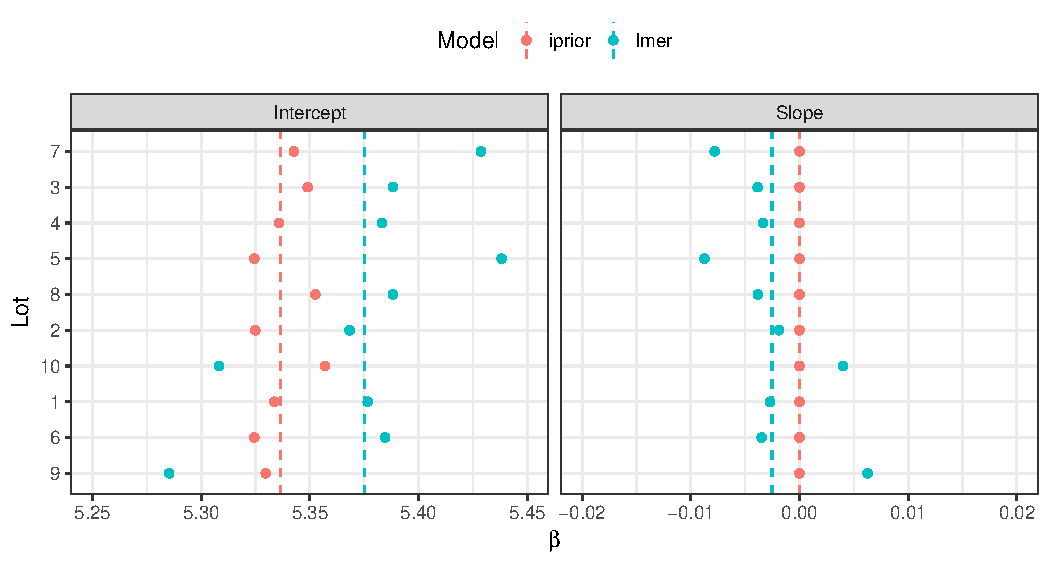
\includegraphics[width=\maxwidth]{figure/04-IGF_plot_beta-1} 

}

\caption[A comparison of the estimates for random intercepts and slopes (denoted as points) using the I-prior model and the standard random effects model]{A comparison of the estimates for random intercepts and slopes (denoted as points) using the I-prior model and the standard random effects model. The dashed vertical lines indicate the fixed effect values.}\label{fig:IGF.plot.beta}
\end{figure}


\end{knitrout}

Degenerate covariance matrices often occur in models with a large number of random coefficients, and in cases where values of the variance components are estimated at the boundary.
These are typically solved by setting restrictions which then avoids overparameterising the model.
One advantage of the I-prior method for varying intercept/slopes model is that the positive-definiteness is automatically taken care of.
Furthermore, I-prior models typically require less number of parameters to fit a similar varying intercept/slopes model -- in the above example, the I-prior model estimated only three parameters, while the standard random effects model estimated a total of six parameters.

It is also possible to ``recover'' the estimates of the standard random effects model from the I-prior model, albeit in a slighly manual fashion (refer to \cref{sec:multilevelmodels}).
Denote by $f^j$ the individual linear regression lines for each of the $j=1,\dots,10$ \code{Lots}.
Then, each of these $f^j$ has a slope and intercept for which we can estimate from the fitted values $\hat f^j(x_{ij})$, $i=1,\dots,n_j$.
This would give us the estimate of the posterior mean of the random intercepts and slopes; these would typically be obtained using empirical-Bayes methods in the case of the standard random effects model.

Furthermore, $\sigma_0^2$ and $\sigma_1^2$ gives a measure of variability of the intercepts and slopes of the different groups, and this can be calculated from the estimates of the random intercepts and slopes.
In the same spirit, $\rho_{01} = \sigma_{01} / (\sigma_0 \sigma_1)$, which is the correlation between the random intercept and slope, can be similarly calculated.
Finally, the fixed effects can be estimated from the intercept and slope of the best fit line running through the I-prior estimated \code{conc} values.
The intuition for this is that the fixed effects are essentially the ordinary least squares (OLS) of a linear model if the groupings are disregarded.
\cref{fig:IGF.plot.beta} illustrates the differences in the estimates for the random coefficients, while  \cref{tab:igf} illustrates the differences in the estimates for the covariance matrix.
Minor differences do exist, with the most noticeable one being that the slopes in the I-prior model are categorically estimated as zero, and the sign of the correlation $\rho_{01}$ being opposite in both models.
Even so, the conclusions from both models are similar.

\begin{table}[htb]
\centering
\caption{A comparison of the estimates for the covariance matrix of the random effects using the I-prior model and the standard random effects model.}
\label{tab:igf}
\begin{tabular}{lrr}
\toprule
Parameter     & \texttt{iprior} & \texttt{lmer} \\
\midrule
$\sigma_0$    & 0.012 & 0.083 \\
$\sigma_1$    & 0.000 & 0.008 \\
$\rho_{01}$   & 0.690& -1.000 \\
\bottomrule
\end{tabular}
\end{table}

\subsection{Longitudinal data analysis}
\label{sec:cows}

We consider a balanced longitudinal data set consisting of weights in kilograms of 60 cows, 30 of which were randomly assigned to treatment group A, and the remaining 30 to treatment group B.
The animals were weighed 11 times over a 133-day period; the first 10 measurements for each animal were made at two-week intervals and the last measurement was made one week later.
This experiment was reported by \citet{kenward1987method}, and the data set is included as part of the package \pkg{jmcm} \citep{jmcm} in \proglang{R}.
The variable names have been renamed for convenience.

\begin{knitrout}
\definecolor{shadecolor}{rgb}{1, 1, 1}\color{fgcolor}\begin{kframe}
\begin{alltt}
\hlstd{R> }\hlkwd{data}\hlstd{(cattle,} \hlkwc{package} \hlstd{=} \hlstr{"jmcm"}\hlstd{)}
\hlstd{R> }\hlkwd{names}\hlstd{(cattle)} \hlkwb{<-} \hlkwd{c}\hlstd{(}\hlstr{"id"}\hlstd{,} \hlstr{"time"}\hlstd{,} \hlstr{"group"}\hlstd{,} \hlstr{"weight"}\hlstd{)}
\hlstd{R> }\hlstd{cattle}\hlopt{$}\hlstd{id} \hlkwb{<-} \hlkwd{as.factor}\hlstd{(cattle}\hlopt{$}\hlstd{id)}  \hlcom{# convert to factors}
\hlstd{R> }\hlkwd{levels}\hlstd{(cattle}\hlopt{$}\hlstd{group)} \hlkwb{<-} \hlkwd{c}\hlstd{(}\hlstr{"Treatment A"}\hlstd{,} \hlstr{"Treatment B"}\hlstd{)}
\hlstd{R> }\hlkwd{str}\hlstd{(cattle)}
\end{alltt}
\begin{verbatim}
## 'data.frame':	660 obs. of  4 variables:
##  $ id    : Factor w/ 60 levels "1","2","3","4",..: 1 1 1 1 1 1 1 1 1..
##  $ time  : num  0 14 28 42 56 70 84 98 112 126 ...
##  $ group : Factor w/ 2 levels "Treatment A",..: 1 1 1 1 1 1 1 1 1 1 ..
##  $ weight: int  233 224 245 258 271 287 287 287 290 293 ...
\end{verbatim}
\end{kframe}
\end{knitrout}

The response variable of interest are the \code{weight} growth curves, and the aim is to investigate whether a treatment effect is present.
The usual approach to analyse a longitudinal data set such as this one is to assume that the observed growth curves are realizations of a Gaussian process.
For example, \citet{kenward1987method} assumed a so-called ante-dependence structure of order $k$, which assumes an observation depends on the previous $k$ observations, but given these, is independent of any preceeding observations.

Using the I-prior, it is not necessary to assume the growth curves were drawn randomly.
Instead, it suffices to assume that they lie in an appropriate function class.
For this example, we assume that the function class is the fBm RKHS, i.e., we assume a smooth effect of time on weight.
The growth curves form a multidimensional (or functional) response equivalent to a ``wide'' format of representing repeated measures data. In our analysis using the \pkg{iprior} package, we used the ``long'' format and thus our (unidimensional) sample size $n$ is equal to $60$ cows $\times$ $11$ repeated measurements.
We also have two covariates potentially influencing growth, namely the cow subject \code{id} and also treatment \code{group}. The regression model can then be thought of as
%
\begin{align*}
  \begin{gathered}
    \text{\code{weight}} = \alpha + f(\text{\code{id}}, \, \text{\code{group}}, \, \text{\code{time}}) + \epsilon \\
    \epsilon \sim \N(0, \psi^{-1}).
  \end{gathered}
\end{align*}
%
\begin{table}[t!]
\centering
\caption{A brief description of the five models fitted using I-priors.}
\label{tab:cowmodel}
\begin{tabular}{lp{6cm}l}
\toprule
Model & Explanation & Formula (\verb@weight ~ ...@) \\
\midrule
1     & Growth does not vary with treatment nor among cows
&\verb@time@ \\
2     & Growth varies among cows only
&\verb@id * time@ \\
3     & Growth varies with treatment only
&\verb@group * time@ \\
4     & Growth varies with treatment and among cows
&\verb@id * time + group * time@ \\
5     & Growth varies with treatment and among cows, with an interaction effect between treatment and cows
&\verb@id * group * time@ \\
\bottomrule
\end{tabular}
\end{table}

\vspace{-1em}
We assume iid errors, and in addition to a smooth effect of \code{time}, we further assume a nominal effect of both cow \code{id} and treatment \code{group} using the Pearson RKHS.
In the \pkg{iprior} package, factor type objects are treated with the Pearson kernel automatically, and the only \code{model} option we need to specify is the \code{kernel = "fbm"} option for the \code{time} variable.
We have opted not to estimate the Hurst coefficient in the interest of computational time, and instead left it at the default value of 0.5.
\cref{tab:cowmodel} explains the five models we have fitted.

The simplest model fitted was one in which the growth curves do not depend on the treatment effect or individual cows.
We then added treatment effect and the cow \code{id} as covariates, separately first and then together at once.
We also assumed that both of these covariates are time-varying, and hence added also the interaction between these covariates and the \code{time} variable.
The final model was one in which an interaction between treatment effect and individual cows was assumed, which varied over time.

All models were fitted using the \code{mixed} estimation method.
Compared to the EM algorithm alone, we found that the combination of direct optimisation with the EM algorithm fits the model about six times faster for this data set due to slow convergence of EM algorithm.
Here is the code and output for fitting the first model:

\begin{knitrout}
\definecolor{shadecolor}{rgb}{1, 1, 1}\color{fgcolor}\begin{kframe}
\begin{alltt}
\hlstd{R> }\hlcom{# Model 1: weight ~ f(time)}
\hlstd{R> }\hlkwd{set.seed}\hlstd{(}\hlnum{456}\hlstd{)}
\hlstd{R> }\hlstd{(mod1} \hlkwb{<-} \hlkwd{iprior}\hlstd{(weight} \hlopt{~} \hlstd{time, cattle,} \hlkwc{kernel} \hlstd{=} \hlstr{"fbm"}\hlstd{,} \hlkwc{method} \hlstd{=} \hlstr{"mixed"}\hlstd{))}
\end{alltt}
\begin{verbatim}
## Running 5 initial EM iterations
## ======================================================================
## Now switching to direct optimisation
## final  value 1394.615062 
## converged
## Log-likelihood value: -2789.231 
## 
##  lambda     psi 
## 0.83592 0.00375
\end{verbatim}
\end{kframe}
\end{knitrout}


\newcolumntype{R}[1]{>{\raggedleft\arraybackslash}p{#1}}
\begin{table}[t!]
\centering
\caption[Summary of the five I-prior models fitted to the cow data set.]{Summary of the five I-prior models fitted to the cow data set. Error S.D. refers to the inverse square root of the error precision, $\psi^{-1/2}$.}
\label{tab:cowresults}
\begin{tabular}{rp{4.9cm}R{2.3cm}R{1.9cm}R{2.2cm}}
\toprule
{\small Model}
& {\small{Formula \newline (}\verb@weight ~ ...@{)}}
& {\small{Log-likelihood}}
& {\small{Error S.D.}}
& {\small{Number of parameters}}  \\
\midrule
1 & \code{time}
& -2789.23
& 16.33
& 1 \\
2 & \code{id * time}
& -2791.42
& 16.39
& 2 \\
3 & \code{group * time}
& -2295.16
& 3.68
& 2 \\
4 & \code{id * time + group * time}
& -2270.85
& 3.39
& 3 \\
5 & \code{id * group * time}
& -2249.26
& 3.90
& 3 \\
\bottomrule
\end{tabular}
\end{table}


The results of the model fit are summarised in \cref{tab:cowresults}. We can test for a treatment effect by testing Model 4 against the alternative that Model 2 is true.
The log-likelihood ratio test statistic is
$D = -2(-2791.42 - (-2270.85)) = 1041.14$, which has an asymptotic chi-squared distribution with $3 - 2 = 1$ degree of freedom.
The $p$-value for this likelihood ratio test is less than $10^{-6}$, so we conclude that Model 4 is significantly better.

We can next investigate whether the treatment effect differs among cows by comparing Model 5 against Model 4.
As these models have the same number of parameters, we can simply choose the one with the higher likelihood, which is Model 5.
We conclude that treatment does indeed have an effect on growth, and that the treatment effect differs among cows.
A plot of the fitted regression curves onto the cow data set is shown in \cref{fig:cows.plot}.

\begin{knitrout}
\definecolor{shadecolor}{rgb}{1, 1, 1}\color{fgcolor}\begin{figure}[htb]

{\centering 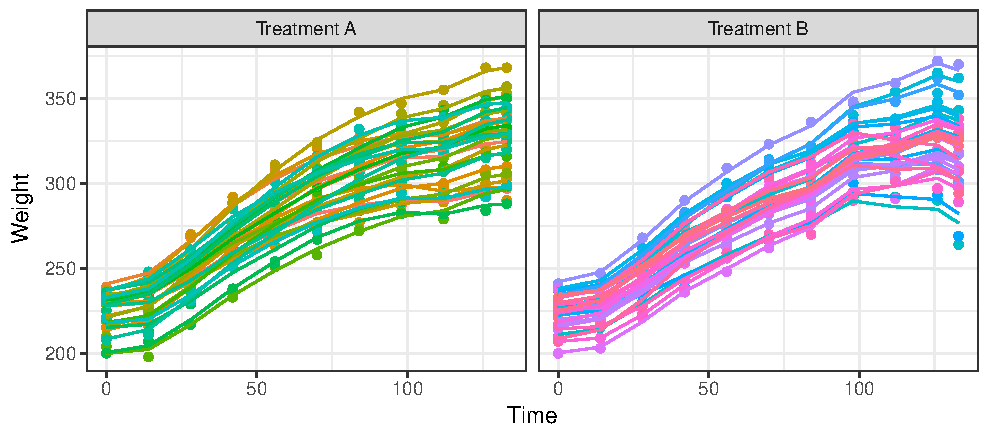
\includegraphics[width=\maxwidth]{figure/04-cows_plot-1} 

}

\caption[A plot of the I-prior fitted regression curves from Model 5]{A plot of the I-prior fitted regression curves from Model 5. In this model, growth curves differ among cows and by treatment effect (with an interaction between cows and treatment effect), thus producing these 60 individual lines, one for each cow, split between their respective treatment groups (A or B).}\label{fig:cows.plot}
\end{figure}


\end{knitrout}

\subsection{Regression with a functional covariate}

We illustrate the prediction of a real valued response with a functional covariate using a widely analysed data set for quality control in the food industry.
The data\footnotemark~contain samples of spectrometric curve of absorbances of 215 pieces of finely chopped meat, along with their water, fat and protein content.
These data are recorded on a Tecator Infratec Food and Feed Analyzer working in the wavelength range 850--1050 nm by the Near Infrared Transmission (NIT) principle.
Absorption data has not been measured continuously, but instead 100 distinct wavelengths were obtained. \cref{fig:tecator.data} shows a sample of 10 such spectrometric curves.

\footnotetext{
Obtained from Tecator (see \url{http://lib.stat.cmu.edu/datasets/tecator} for details).
We used the version made available in the dataframe \code{tecator} from the \proglang{R} package \pkg{caret} \citep{caret}.
}

\begin{knitrout}
\definecolor{shadecolor}{rgb}{1, 1, 1}\color{fgcolor}\begin{figure}[htb]

{\centering 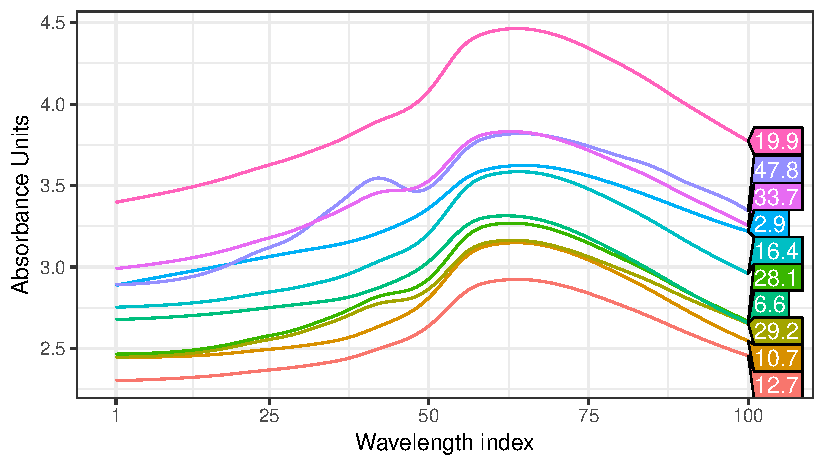
\includegraphics[width=12cm]{figure/04-tecator_data-1} 

}

\caption[Sample of spectrometric curves used to predict fat content of meat]{Sample of spectrometric curves used to predict fat content of meat. For each meat sample the data consists of a 100 channel spectrum of absorbances and the contents of moisture, fat (numbers shown in boxes) and protein measured in percent. The absorbance is $-\log 10$ of the transmittance measured by the spectrometer. The three contents, measured in percent, are determined by analytic chemistry.}\label{fig:tecator.data}
\end{figure}


\end{knitrout}

For our analyses and many others' in the literature, the first 172 observations in the data set are used as a training sample for model fitting, and the remaining 43 observations as a test sample to evaluate the predictive performance of the fitted model.
The focus here is to use the \pkg{iprior} package to fit several I-prior models to the Tecator data set, and calculate out-of-sample predictive error rates.
We compare the predictive performance of I-prior models against Gaussian process regression and the many other different methods applied on this data set.
These methods include neural networks \citep{thodberg1996review}, kernel smoothing \citep{ferraty2006nonparametric}, single and multiple index functional regression models \citep{chen2011single}, sliced inverse regression (SIR) and sliced average variance estimation (SAVE), multivariate adaptive regression splines (MARS), partial least squares (PLS), and functional additive model with and without component selection (FAM \& CSEFAM).
An analysis of this data set using the SIR and SAVE methods were conducted by  \citet{lian2014series}, while the MARS, PLS and (CSE)FAM methods were studied by \citet{zhu2014structured}.
\cref{tab:tecator} tabulates the results of all of these methods from the various references.

Assuming a regression model as in \cref{eq:model2}, we would like to model the \code{fat} content $y_i$ using the spectral curves $x_i$.
Let $x_i(t)$ denote the absorbance for wavelength $t = 1,\dots,100$.
From \cref{fig:tecator.data}, it appears that the curves are smooth enough to be differentiable, and therefore it is reasonable to assume that they lie in the Sobolev-Hilbert space as discussed in \cref{sec:regfunctionalcov}.
We take first differences of the 100-dimensional matrix, which leaves us with the 99-dimensional covariate saved in the object named \code{absorp}.
The \code{fat} and \code{absorp} data have been split into \code{*.train} and \code{*.test} samples, as mentioned earlier.
Our first modelling attempt is to fit a linear effect by regressing the responses \code{fat.train} against a single high-dimensional covariate \code{absorp.train} using the linear RKHS and the direct optimisation method.

\begin{knitrout}
\definecolor{shadecolor}{rgb}{1, 1, 1}\color{fgcolor}\begin{kframe}
\begin{alltt}
\hlstd{R> }\hlcom{# Model 1: Canonical RKHS (linear)}
\hlstd{R> }\hlstd{(mod1} \hlkwb{<-} \hlkwd{iprior}\hlstd{(}\hlkwc{y} \hlstd{= fat.train, absorp.train))}
\end{alltt}
\begin{verbatim}
## iter   10 value 222.653144
## final  value 222.642108 
## converged
## Log-likelihood value: -445.2844 
## 
##     lambda        psi 
## 4576.86595    0.11576
\end{verbatim}
\end{kframe}
\end{knitrout}

Our second and third model uses polynomial RKHSs of degrees two and three, which allows us to model quadratic and cubic terms of the spectral curves respectively.
We also opted to estimate a suitable offset parameter, and this is called to \code{iprior()} with the option \code{est.offset = TRUE}.
Each of the two models has a single scale parameter, an offset parameter, and an error precision to be estimated.
The direct optimisation method has been used, and while both models converged regularly, it was noticed that there were multiple local optima that hindered the estimation (output omitted).

\begin{knitrout}
\definecolor{shadecolor}{rgb}{1, 1, 1}\color{fgcolor}\begin{kframe}
\begin{alltt}
\hlstd{R> }\hlcom{# Model 2: Polynomial RKHS (quadratic)}
\hlstd{R> }\hlstd{mod2} \hlkwb{<-} \hlkwd{iprior}\hlstd{(}\hlkwc{y} \hlstd{= fat.train, absorp.train,} \hlkwc{kernel} \hlstd{=} \hlstr{"poly2"}\hlstd{,}
\hlstd{+  }               \hlkwc{est.offset} \hlstd{=} \hlnum{TRUE}\hlstd{)}
\hlstd{R> }\hlcom{# Model 3: Polynomial RKHS (cubic)}
\hlstd{R> }\hlstd{mod3} \hlkwb{<-} \hlkwd{iprior}\hlstd{(}\hlkwc{y} \hlstd{= fat.train, absorp.train,} \hlkwc{kernel} \hlstd{=} \hlstr{"poly3"}\hlstd{,}
\hlstd{+  }               \hlkwc{est.offset} \hlstd{=} \hlnum{TRUE}\hlstd{)}
\end{alltt}
\end{kframe}
\end{knitrout}

Next, we attempt to fit a smooth dependence of fat content on the spectrometric curves using the fBm RKHS.
By default, the Hurst coefficient for the fBm RKHS is set to be 0.5.
However, with the option \code{est.hurst = TRUE}, the Hurst coefficient is included in the estimation procedure.
We fit models with both a fixed value for Hurst (at 0.5) and an estimated value for Hurst.
For both of these models, we encountered numerical issues when using the direct optimisation method.
The L-BFGS algorithm kept on pulling the hyperparameter towards extremely high values, which in turn made the log-likelihood value greater than the machine's largest normalised floating-point number (\code{.Machine$double.xmax = 1.797693e+308}).
% Investigating further, it seems that estimates at these large values give poor training and test error rates, though likelihood values here are high (local optima).
To circumvent this issue, we used the EM algorithm to estimate the fixed Hurst model, and the \code{mixed} method for the estimated Hurst model.
For both models, the \code{stop.crit} was relaxed and set to \code{1e-3} for quicker convergence, though this did not affect the predictive abilities compared to a more stringent \code{stop.crit}.

\begin{knitrout}
\definecolor{shadecolor}{rgb}{1, 1, 1}\color{fgcolor}\begin{kframe}
\begin{alltt}
\hlstd{R> }\hlcom{# Model 4: fBm RKHS (default Hurst = 0.5)}
\hlstd{R> }\hlstd{(mod4} \hlkwb{<-} \hlkwd{iprior}\hlstd{(}\hlkwc{y} \hlstd{= fat.train, absorp.train,} \hlkwc{kernel} \hlstd{=} \hlstr{"fbm"}\hlstd{,}
\hlstd{+  }                \hlkwc{method} \hlstd{=} \hlstr{"em"}\hlstd{,} \hlkwc{control} \hlstd{=} \hlkwd{list}\hlstd{(}\hlkwc{stop.crit} \hlstd{=} \hlnum{1e-3}\hlstd{)))}
\end{alltt}
\begin{verbatim}
## ==============================================
## Converged after 65 iterations.
## Log-likelihood value: -204.4592 
## 
##     lambda        psi 
##    3.24112 1869.32897
\end{verbatim}
\end{kframe}
\end{knitrout}
\begin{knitrout}
\definecolor{shadecolor}{rgb}{1, 1, 1}\color{fgcolor}\begin{kframe}
\begin{alltt}
\hlstd{R> }\hlcom{# Model 5: fBm RKHS (estimate Hurst)}
\hlstd{R> }\hlstd{(mod5} \hlkwb{<-} \hlkwd{iprior}\hlstd{(fat.train, absorp.train,} \hlkwc{kernel} \hlstd{=} \hlstr{"fbm"}\hlstd{,} \hlkwc{method} \hlstd{=} \hlstr{"mixed"}\hlstd{,}
\hlstd{+  }                \hlkwc{est.hurst} \hlstd{=} \hlnum{TRUE}\hlstd{,} \hlkwc{control} \hlstd{=} \hlkwd{list}\hlstd{(}\hlkwc{stop.crit} \hlstd{=} \hlnum{1e-3}\hlstd{)))}
\end{alltt}
\begin{verbatim}
## Running 5 initial EM iterations
## ======================================================================
## Now switching to direct optimisation
## iter   10 value 115.648462
## final  value 115.645800 
## converged
## Log-likelihood value: -231.2923 
## 
##    lambda     hurst       psi 
## 204.97184   0.70382   9.96498
\end{verbatim}
\end{kframe}
\end{knitrout}

Finally, we fit an I-prior model using the SE RKHS with lengthscale estimated.
Here we illustrate the use of the \code{restarts} option, in which the model is fitted repeatedly from different starting points.
In this case, eight random initial parameter values were used and these jobs were parallelised across the eight available cores of the machine.
The additional \code{par.maxit} option in the \code{control} list is an option for the maximum number of iterations that each parallel job should do.
We have set it to 100, which is the same number for \code{maxit}, but if \code{par.maxit} is less than \code{maxit}, the estimation procedure continues from the model with the best likelihood value.
We see that starting from eight different initial values, direct optimisation leads to (at least) two log-likelihood optima sites, $-231.5$ and $-680.5$.

\begin{knitrout}
\definecolor{shadecolor}{rgb}{1, 1, 1}\color{fgcolor}\begin{kframe}
\begin{alltt}
\hlstd{R> }\hlcom{# Model 6: SE kernel}
\hlstd{R> }\hlstd{(mod6} \hlkwb{<-} \hlkwd{iprior}\hlstd{(fat.train, absorp.train,} \hlkwc{est.lengthscale} \hlstd{=} \hlnum{TRUE}\hlstd{,}
\hlstd{+  }                \hlkwc{kernel} \hlstd{=} \hlstr{"se"}\hlstd{,} \hlkwc{control} \hlstd{=} \hlkwd{list}\hlstd{(}\hlkwc{restarts} \hlstd{=} \hlnum{TRUE}\hlstd{,}
\hlstd{+  }                                              \hlkwc{par.maxit} \hlstd{=} \hlnum{100}\hlstd{)))}
\end{alltt}
\begin{verbatim}
## Performing 8 random restarts on 8 cores
## ======================================================================
## Log-likelihood from random starts:
##     Run 1     Run 2     Run 3     Run 4     Run 5     Run 6     Run 7 
## -231.5440 -680.4636 -680.4636 -680.4637 -680.4637 -231.5440 -231.5440 
## Continuing on Run 6 
## final  value 115.771932 
## converged
## Log-likelihood value: -231.544 
## 
##      lambda lengthscale         psi 
##    96.11515     0.09269     6.15426
\end{verbatim}
\end{kframe}
\end{knitrout}



% \renewcommand{\TPTminimum}{0.5\linewidth}
\newcolumntype{R}[1]{>{\raggedleft\arraybackslash}p{#1}}
\begin{table}[p]
\centering
\caption{A summary of the root mean squared error (RMSE) of prediction for the I-prior models and various other methods in literature conducted on the Tecator data set. Values for the methods under \emph{Others} were obtained from the corresponding references cited earlier.}
\label{tab:tecator}
\begin{threeparttable}
% \begin{tabular}{@{}p{\textwidth}@{}}
\begin{tabular}{p{7cm}rr}
\toprule
\Bot &\multicolumn{2}{c}{RMSE} \\
\cline{2-3}
\Top Model & Train & Test \\
\midrule
\emph{I-prior} \\
\hspace{0.5em} Linear
& 2.89
& 2.89 \\
\hspace{0.5em} Quadratic
& 0.72
& 0.97 \\
\hspace{0.5em} Cubic
& 0.37
& 0.58 \\
\hspace{0.5em} Smooth (fBm-0.50)
& 0.00
& 0.68 \\
\hspace{0.5em} Smooth (fBm-0.70)
& 0.19
& 0.63 \\
\hspace{0.5em} Smooth (SE-0.09)
& 0.35
& 1.85 \\
\\
\emph{Gaussian process regression} \\
\hspace{0.5em} Linear
& 0.18
& 2.36 \\
\hspace{0.5em} Smooth (SE-7.04)
& 0.17
& 2.10 \\
\\
\emph{Others} \\
%\hspace{0.5em} Linear functional regression\tnote{a}       && 2.78 \\
%\hspace{0.5em} Quadratic functional regression\tnote{a}    && 0.80 \\
\hspace{0.5em} Neural network\tnote{a}                     && 0.36 \\
\hspace{0.5em} Kernel smoothing\tnote{b}                   && 1.49 \\
\hspace{0.5em} Single/multiple indices model\tnote{c}      && 1.55 \\
\hspace{0.5em} Sliced inverse regression                   && 0.90 \\
\hspace{0.5em} Sliced average variance estimation          && 1.70 \\
\hspace{0.5em} MARS\tnote{d}                               && 0.88 \\
\hspace{0.5em} Partial least squares\tnote{d}              && 1.01 \\
%\hspace{0.5em} FAM\tnote{d}                                && 0.92 \\
\hspace{0.5em} CSEFAM\tnote{d}                             && 0.85 \\
\bottomrule
\end{tabular}
% \end{tabular}
\begin{tablenotes}\footnotesize
\item [a] Neural network best results with automatic relevance determination (ARD) quoted.
\item [b] Data set used was a 160/55 training/test split.
\item [c] These are results of a leave-one-out cross-validation scheme.
\item [d] Data set used was an extended version with $n=240$, and a random 185/55 training/test split.
\end{tablenotes}
\end{threeparttable}
\end{table}

Predicted values of the test data set can be obtained using the \code{predict()} function.
An example for obtaining the first model's predicted values is shown below.
The \code{predict()} method for \code{ipriorMod} objects also return the test MSE if the vector of test data is supplied.

\begin{knitrout}
\definecolor{shadecolor}{rgb}{1, 1, 1}\color{fgcolor}\begin{kframe}
\begin{alltt}
\hlstd{R> }\hlkwd{predict}\hlstd{(mod1,} \hlkwc{newdata} \hlstd{=} \hlkwd{list}\hlstd{(absorp.test),} \hlkwc{y.test} \hlstd{= fat.test)}
\end{alltt}
\begin{verbatim}
## Test RMSE: 2.890353 
## 
## Predicted values:
##  [1] 43.607 20.444  7.821  4.491  9.044  8.564  7.935 11.615 13.807
## [10] 17.359
## # ... with 33 more values
\end{verbatim}
\end{kframe}
\end{knitrout}

These results are summarised in \cref{tab:tecator}.
For the I-prior models, a linear effect of the functional covariate gives a training RMSE of 2.89, which is improved by both the qudratic and cubic model.
The training RMSE is improved further by assuming a smooth RKHS of functions for $f$, i.e. the fBm and SE RKHSs.
When it comes to out-of-sample test error rates, the cubic model gives the best RMSE out of the I-prior models for this particular data set, with an RMSE of 0.58.
This is followed closely by the fBm RKHS with estimated Hurst coefficient (fBm-0.70) and also the fBm RKHS with default Hurst coefficient (fBm-0.50).
The best performing I-prior model is only outclassed by the neural networks of \citet{thodberg1996review}, who also performed model selection using automatic relevance determination (ARD).
The I-prior models also give much better test RMSE than Gaussian process regression\footnote{GPR models were fit using \texttt{gausspr()} in \pkg{kernlab}.}.
\end{document}


